\documentclass[10pt,letterpaper]{article}
\usepackage[top=1in,bottom=1in,left=1in,right=1in]{geometry}
\usepackage{datetime}
\usepackage{natbib}      % http://merkel.zoneo.net/Latex/natbib.php
\usepackage{palatino}
\usepackage{verbatim}
\usepackage[normalem]{ulem}

\bibpunct{(}{)}{;}{a}{,}{,}

\usepackage{array}

\usepackage{chngpage}
\usepackage{stmaryrd}
\usepackage{amssymb}
\usepackage{amsmath}
\usepackage{graphicx}
\usepackage{lscape}
\usepackage{subfigure}
\usepackage[usenames,dvipsnames]{color}
\definecolor{myblue}{rgb}{0,0.1,0.6}
\definecolor{mygreen}{rgb}{0,0.3,0.1}
\usepackage[colorlinks=true,linkcolor=black,citecolor=mygreen,urlcolor=myblue]{hyperref}

\newcommand{\bocomment}[1]{\textcolor{Bittersweet}{BO says: #1}}

\newcommand{\ignore}[1]{}
\newcommand{\transpose}{^\mathsf{T}}
\newcommand{\inner}[1]{\langle #1 \rangle} 
\newcommand{\smallsec}[1]{\noindent \textbf{#1\ }}
\newcommand{\cmd}[1] {{\color{blue}\texttt{#1}}}

\newcommand{\solution}[1]{{\color{myblue} \emph{[Solution:} 

#1 

\emph{End solution]}}}
\newcommand{\solutionnote}[1]{{\color{myblue} \emph{[Note:}

#1 

\emph{End note]}}}
\newcommand{\points}[1]{{\color{mygreen}\emph{[#1]\ \ }}}

\newcommand{\aone}{\diamondsuit}
\newcommand{\atwo}{\heartsuit}
\newcommand{\bone}{\triangle}
\newcommand{\btwo}{\Box}
\newcommand{\myand}{\ \land\ }
\newcommand{\myor}{\ \lor\ }
\newcommand{\mynot}{\lnot}

\title{
  \textbf{Mini-project 1: Color images Solution} \\
  \textbf{Name: Abhay Doke}\\
  \textbf{UID:29552668}
}

\settimeformat{ampmtime}
\date{}
\begin{document}
\maketitle

\section{Aligning Prokudin-Gorskii images - Aligned output images} 
For aligning the Prokudin-Gorskii images I have used their edge information for calculating Sum of Squared Differences (SSD) distances.
Canny edge detector is used for finding edges in images. Using edge information gives better results than just using the raw pixels.
All the images can be found in the \textbf{output/prokudin-gorskii/} folder.\newline
For the first problem in the assignment images are smaller in size and hence processing with the shift window size of [15,15] is quick. But for the larger images given in the Extension exercise, processing with this window size was slow. Hence I used an image pyramid which scales down the bigger image multiple times. A small window size is then used to predict the shift. This shift is applied to the next large image in the pyramid. This version works faster for the large images. Results of these large images can be found in the \textbf{output/large-images/} folder.\newline\newline

Results of the aligned Prokudin images:
\begin{figure}
\centering
\mbox{\subfigure{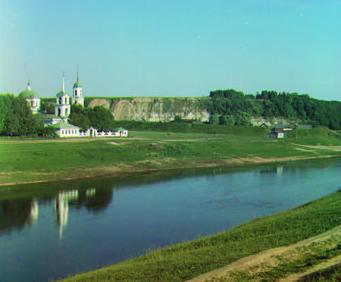
\includegraphics[width=3in]{../output/prokudin-gorskii/00125-aligned.jpg}}\quad
\subfigure{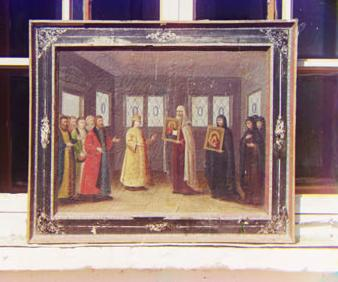
\includegraphics[width=3in]{../output/prokudin-gorskii/00149-aligned.jpg} }}
\end{figure}

\begin{figure}
\centering
\mbox{\subfigure{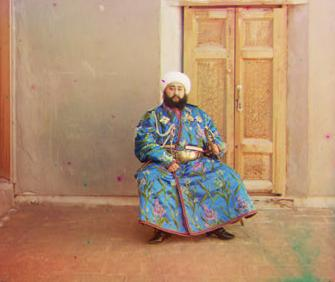
\includegraphics[width=3in]{../output/prokudin-gorskii/00153-aligned.jpg}}\quad
\subfigure{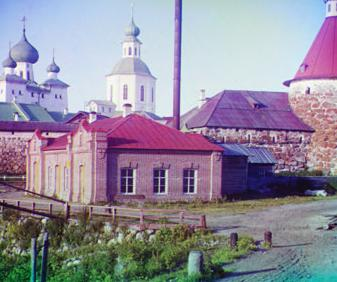
\includegraphics[width=3in]{../output/prokudin-gorskii/00351-aligned.jpg} }}
\end{figure}

\begin{figure}
\centering
\mbox{\subfigure{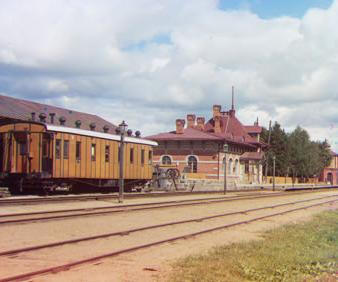
\includegraphics[width=3in]{../output/prokudin-gorskii/00398-aligned.jpg}}\quad
\subfigure{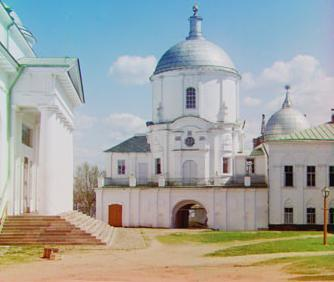
\includegraphics[width=3in]{../output/prokudin-gorskii/01112-aligned.jpg} }}
\end{figure}

\newpage
Below is the code of the \textbf{alignChannels.m}\newline
\verbatiminput{alignChannels.m}

\newpage
Result of the \textbf{evalAlignment.m}\newline
\verbatiminput{evalOutput.txt}

Computed shifts for each of the Prokudin images\newline
\verbatiminput{alignProkudinOutput.txt}

\newpage
\section{Color image demosaicing}
Below is the code of the \textbf{demosaicimage.m}\newline
\verbatiminput{demosaicimage.m}

Result of the \textbf{evalDemosaic.m}\newline
\verbatiminput{evalDemosaicOutput.txt}

I have described the implementation details using comments in the code describing each step in the code.\newpage



\section{EXTENSION part of the home work -- Aligning Large Prokudin-Gorskii images}
For the larger images given in the Extension exercise, processing with this window size was slow. Hence I used an image pyramid which scales down the bigger image multiple times. A small window size is then used to predict the shift. This shift is applied to the next large image in the pyramid. This version works faster for the large images. Results of these large images can be found in the \textbf{output/large-images/} folder.\newline\newline

Below is the code of the \textbf{alignProkudinNew.m} which makes a image pyramid and then calculates the shifts\newline
\verbatiminput{alignProkudinNew.m}


Results of the alignments are shown below:

\newpage
 
\begin{figure}
\centering
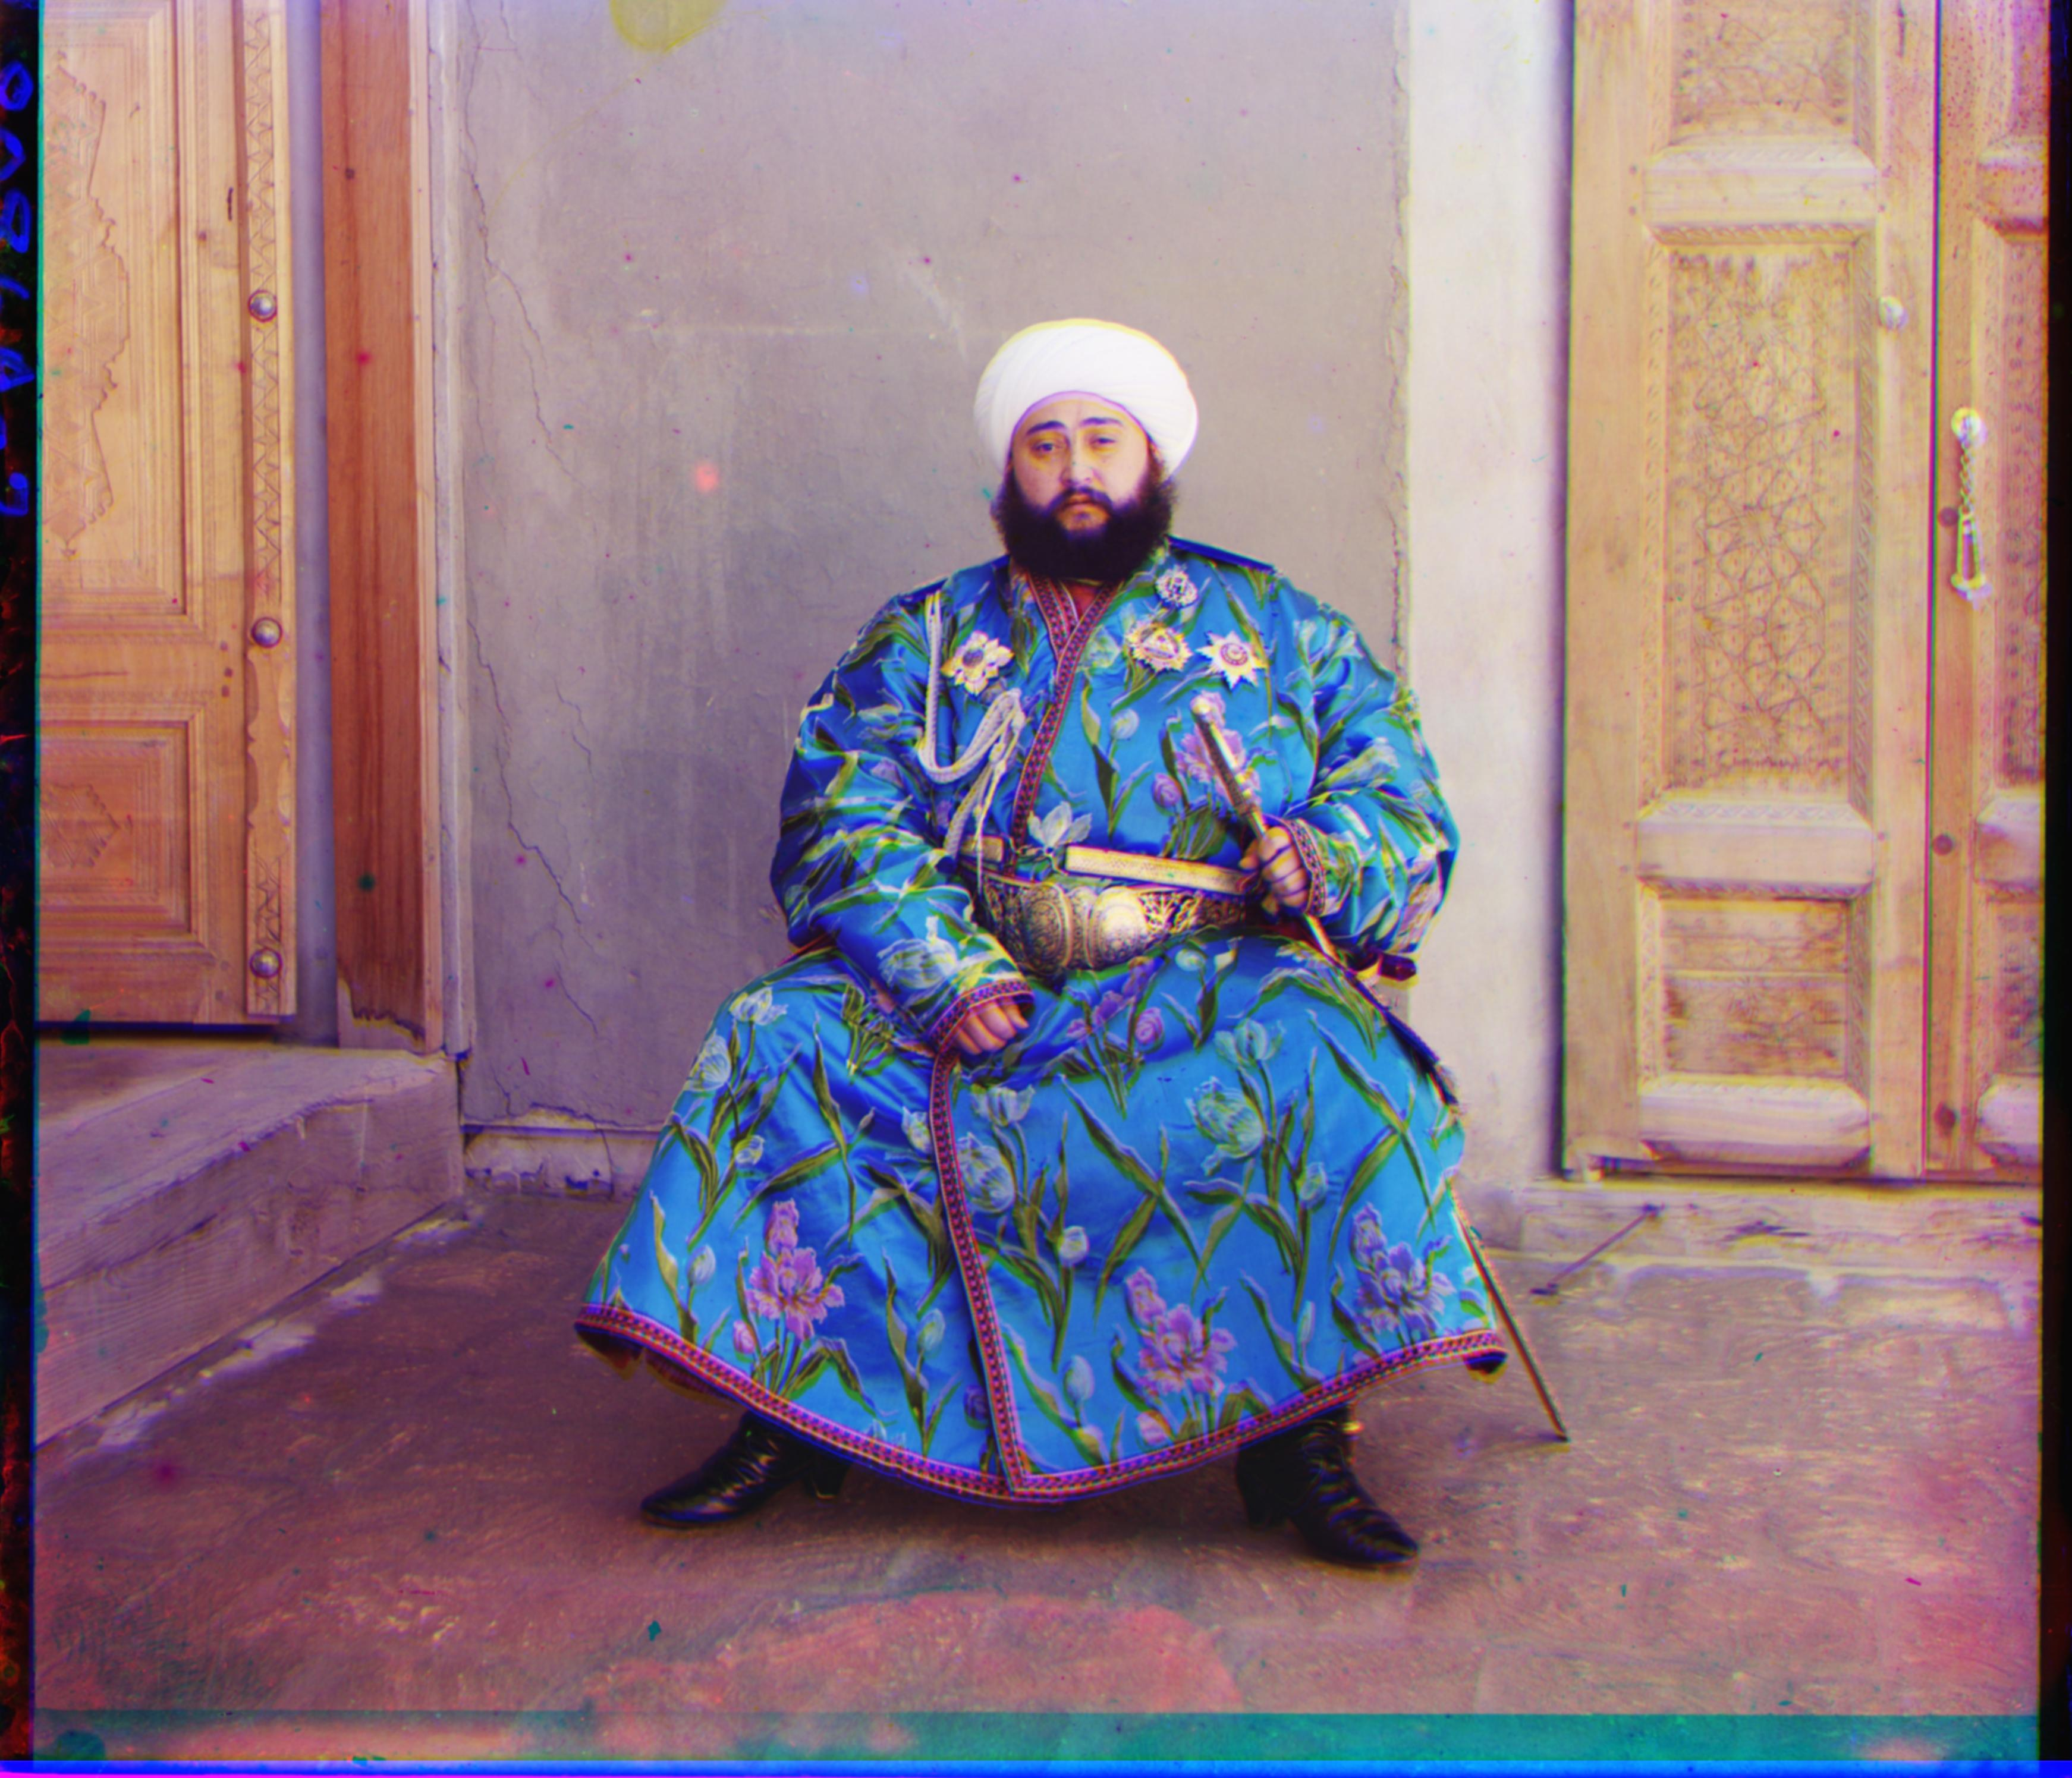
\includegraphics[width=\textwidth,height=\textheight,keepaspectratio]{../output/large-images/emi-aligned.jpg}
\caption{Aligned image for emir.tif  size = 3485 x 2991}
\end{figure}

\begin{figure}
\centering
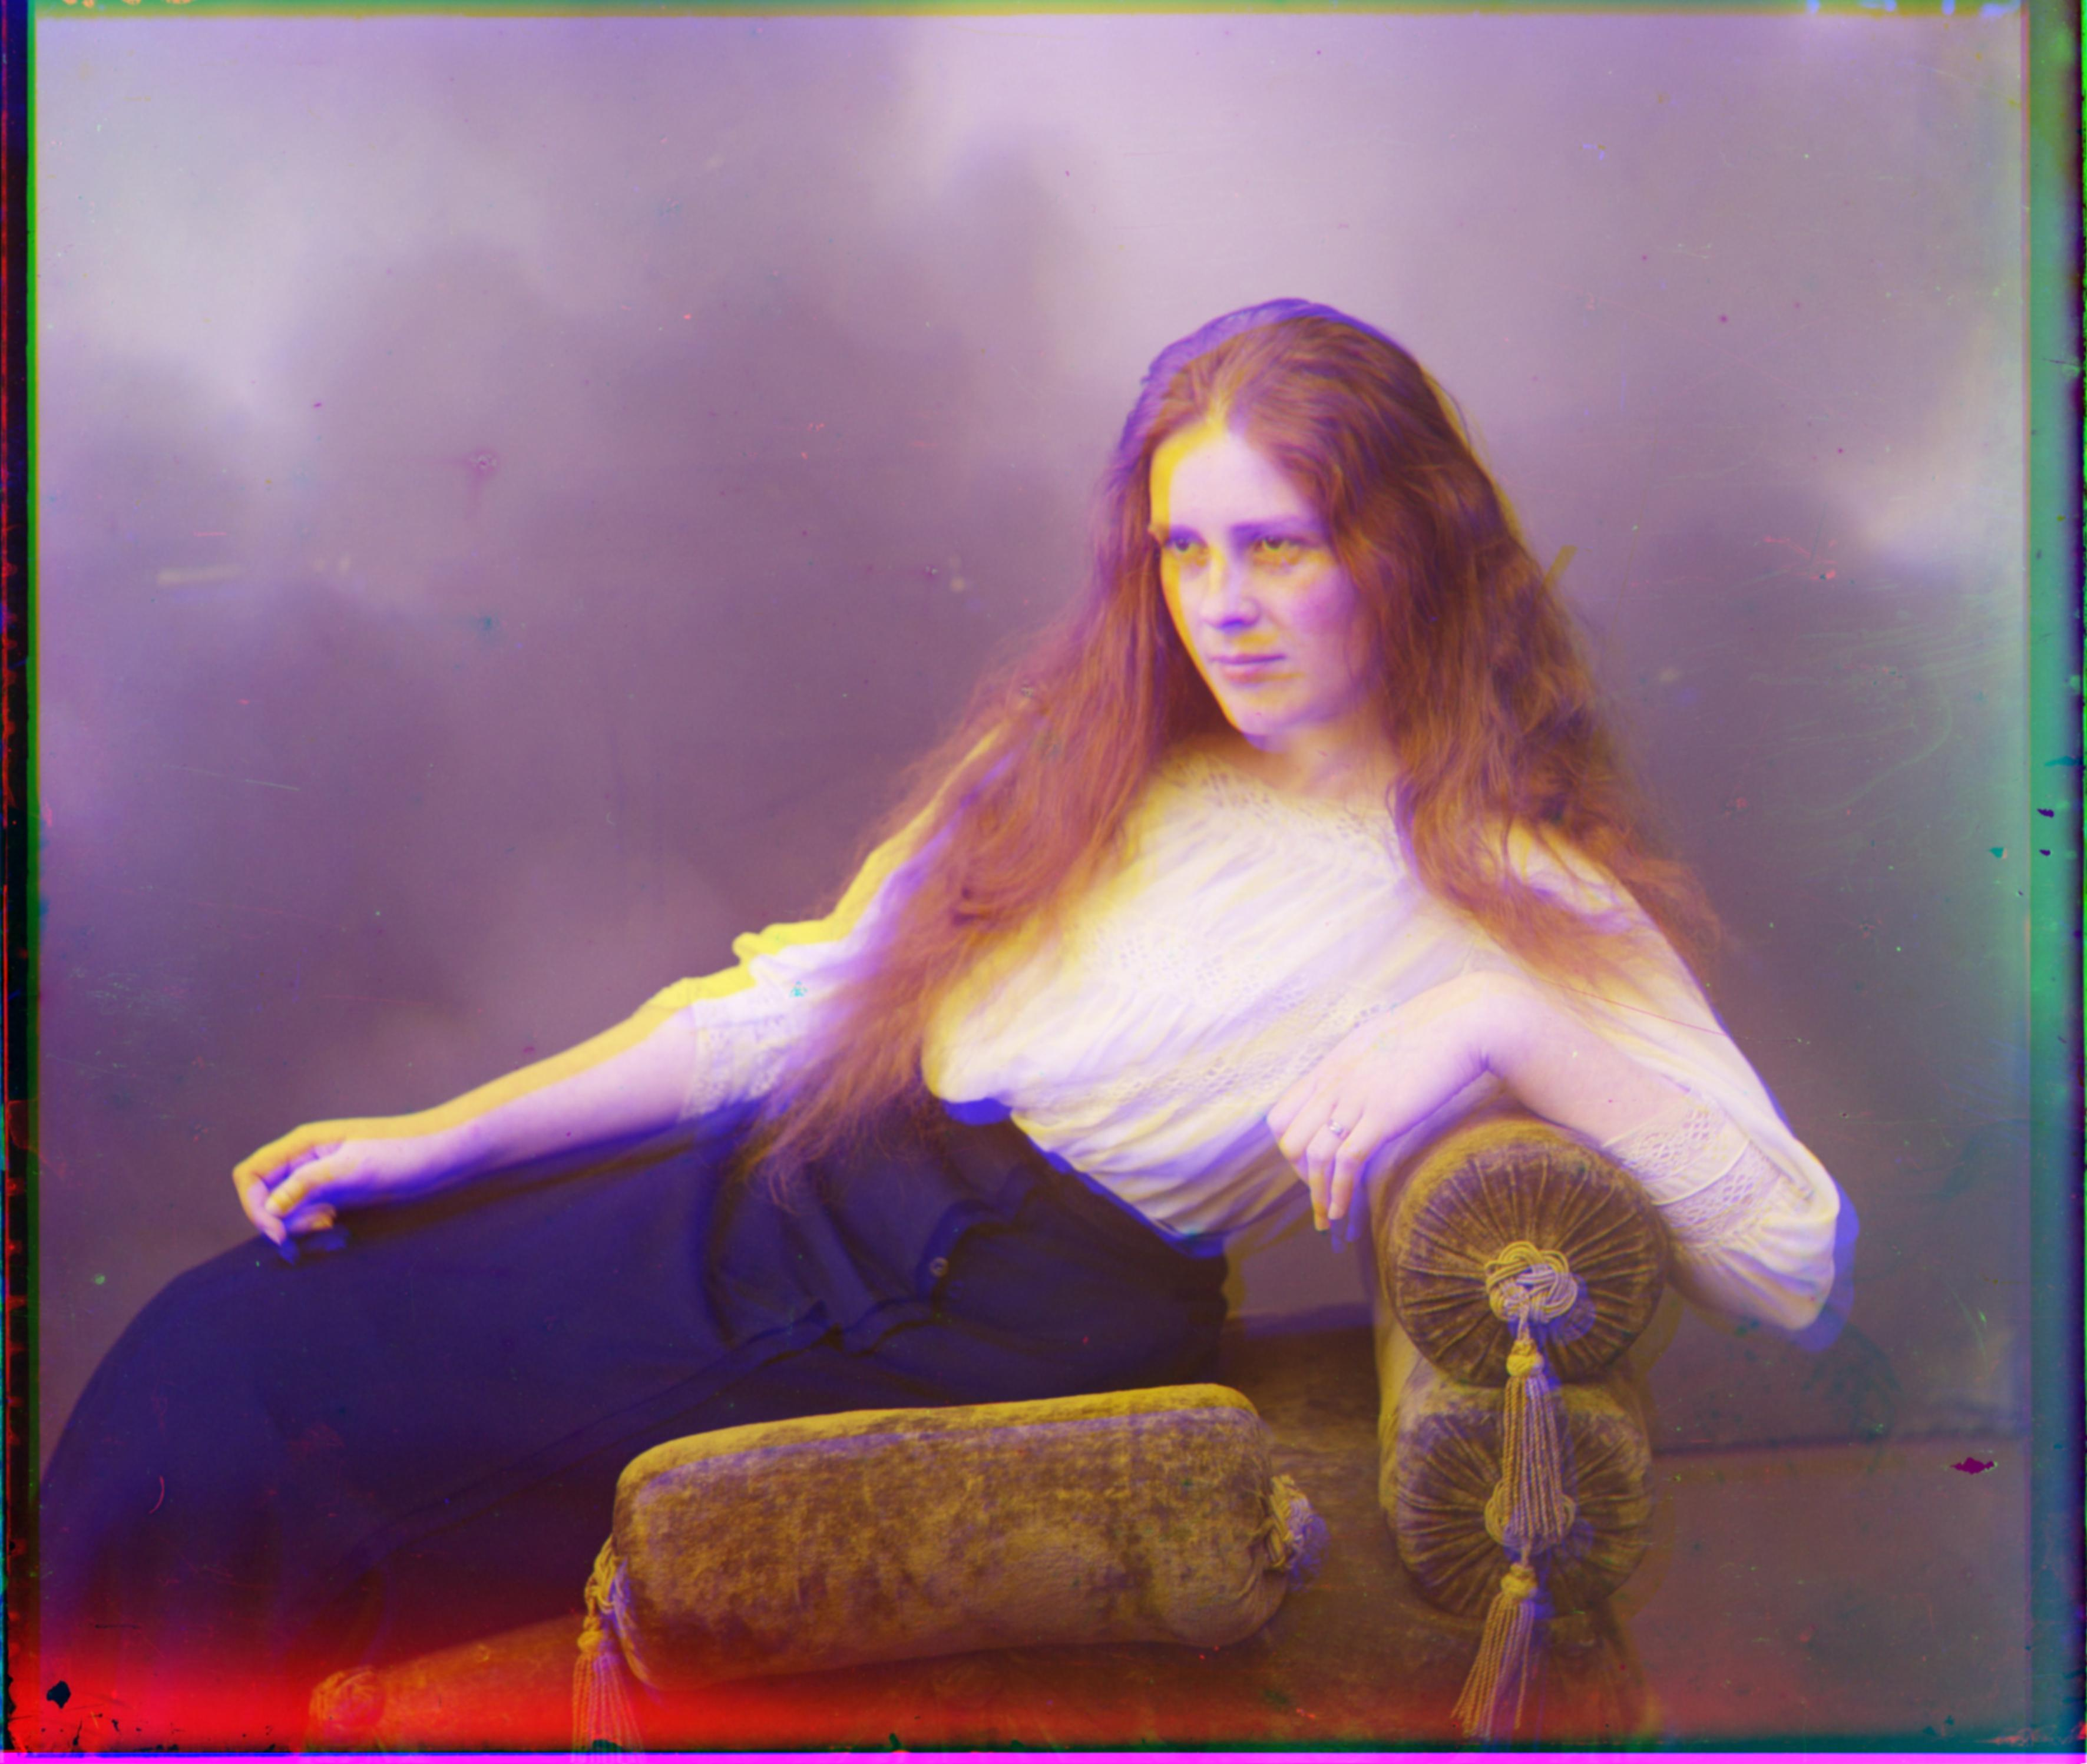
\includegraphics[width=\textwidth,height=\textheight,keepaspectratio]{../output/large-images/lad-aligned.jpg}
\caption{Aligned image for lady.tif size = 3543 x 2995 }
\end{figure}

\begin{figure}
\centering
\includegraphics[width=\textwidth,height=\textheight,keepaspectratio]{../output/large-images/onion-churc-aligned.jpg}
\caption{Aligned image for onion-church.tif  size = 3563 x 2997}
\end{figure}


\begin{figure}
\centering
\includegraphics[width=\textwidth,height=\textheight,keepaspectratio]{../output/large-images/threegenerationsaligned.jpg}
\caption{Aligned image for three-generations.tif  size = 3497 x 2991}
\end{figure}

\begin{figure}
\centering
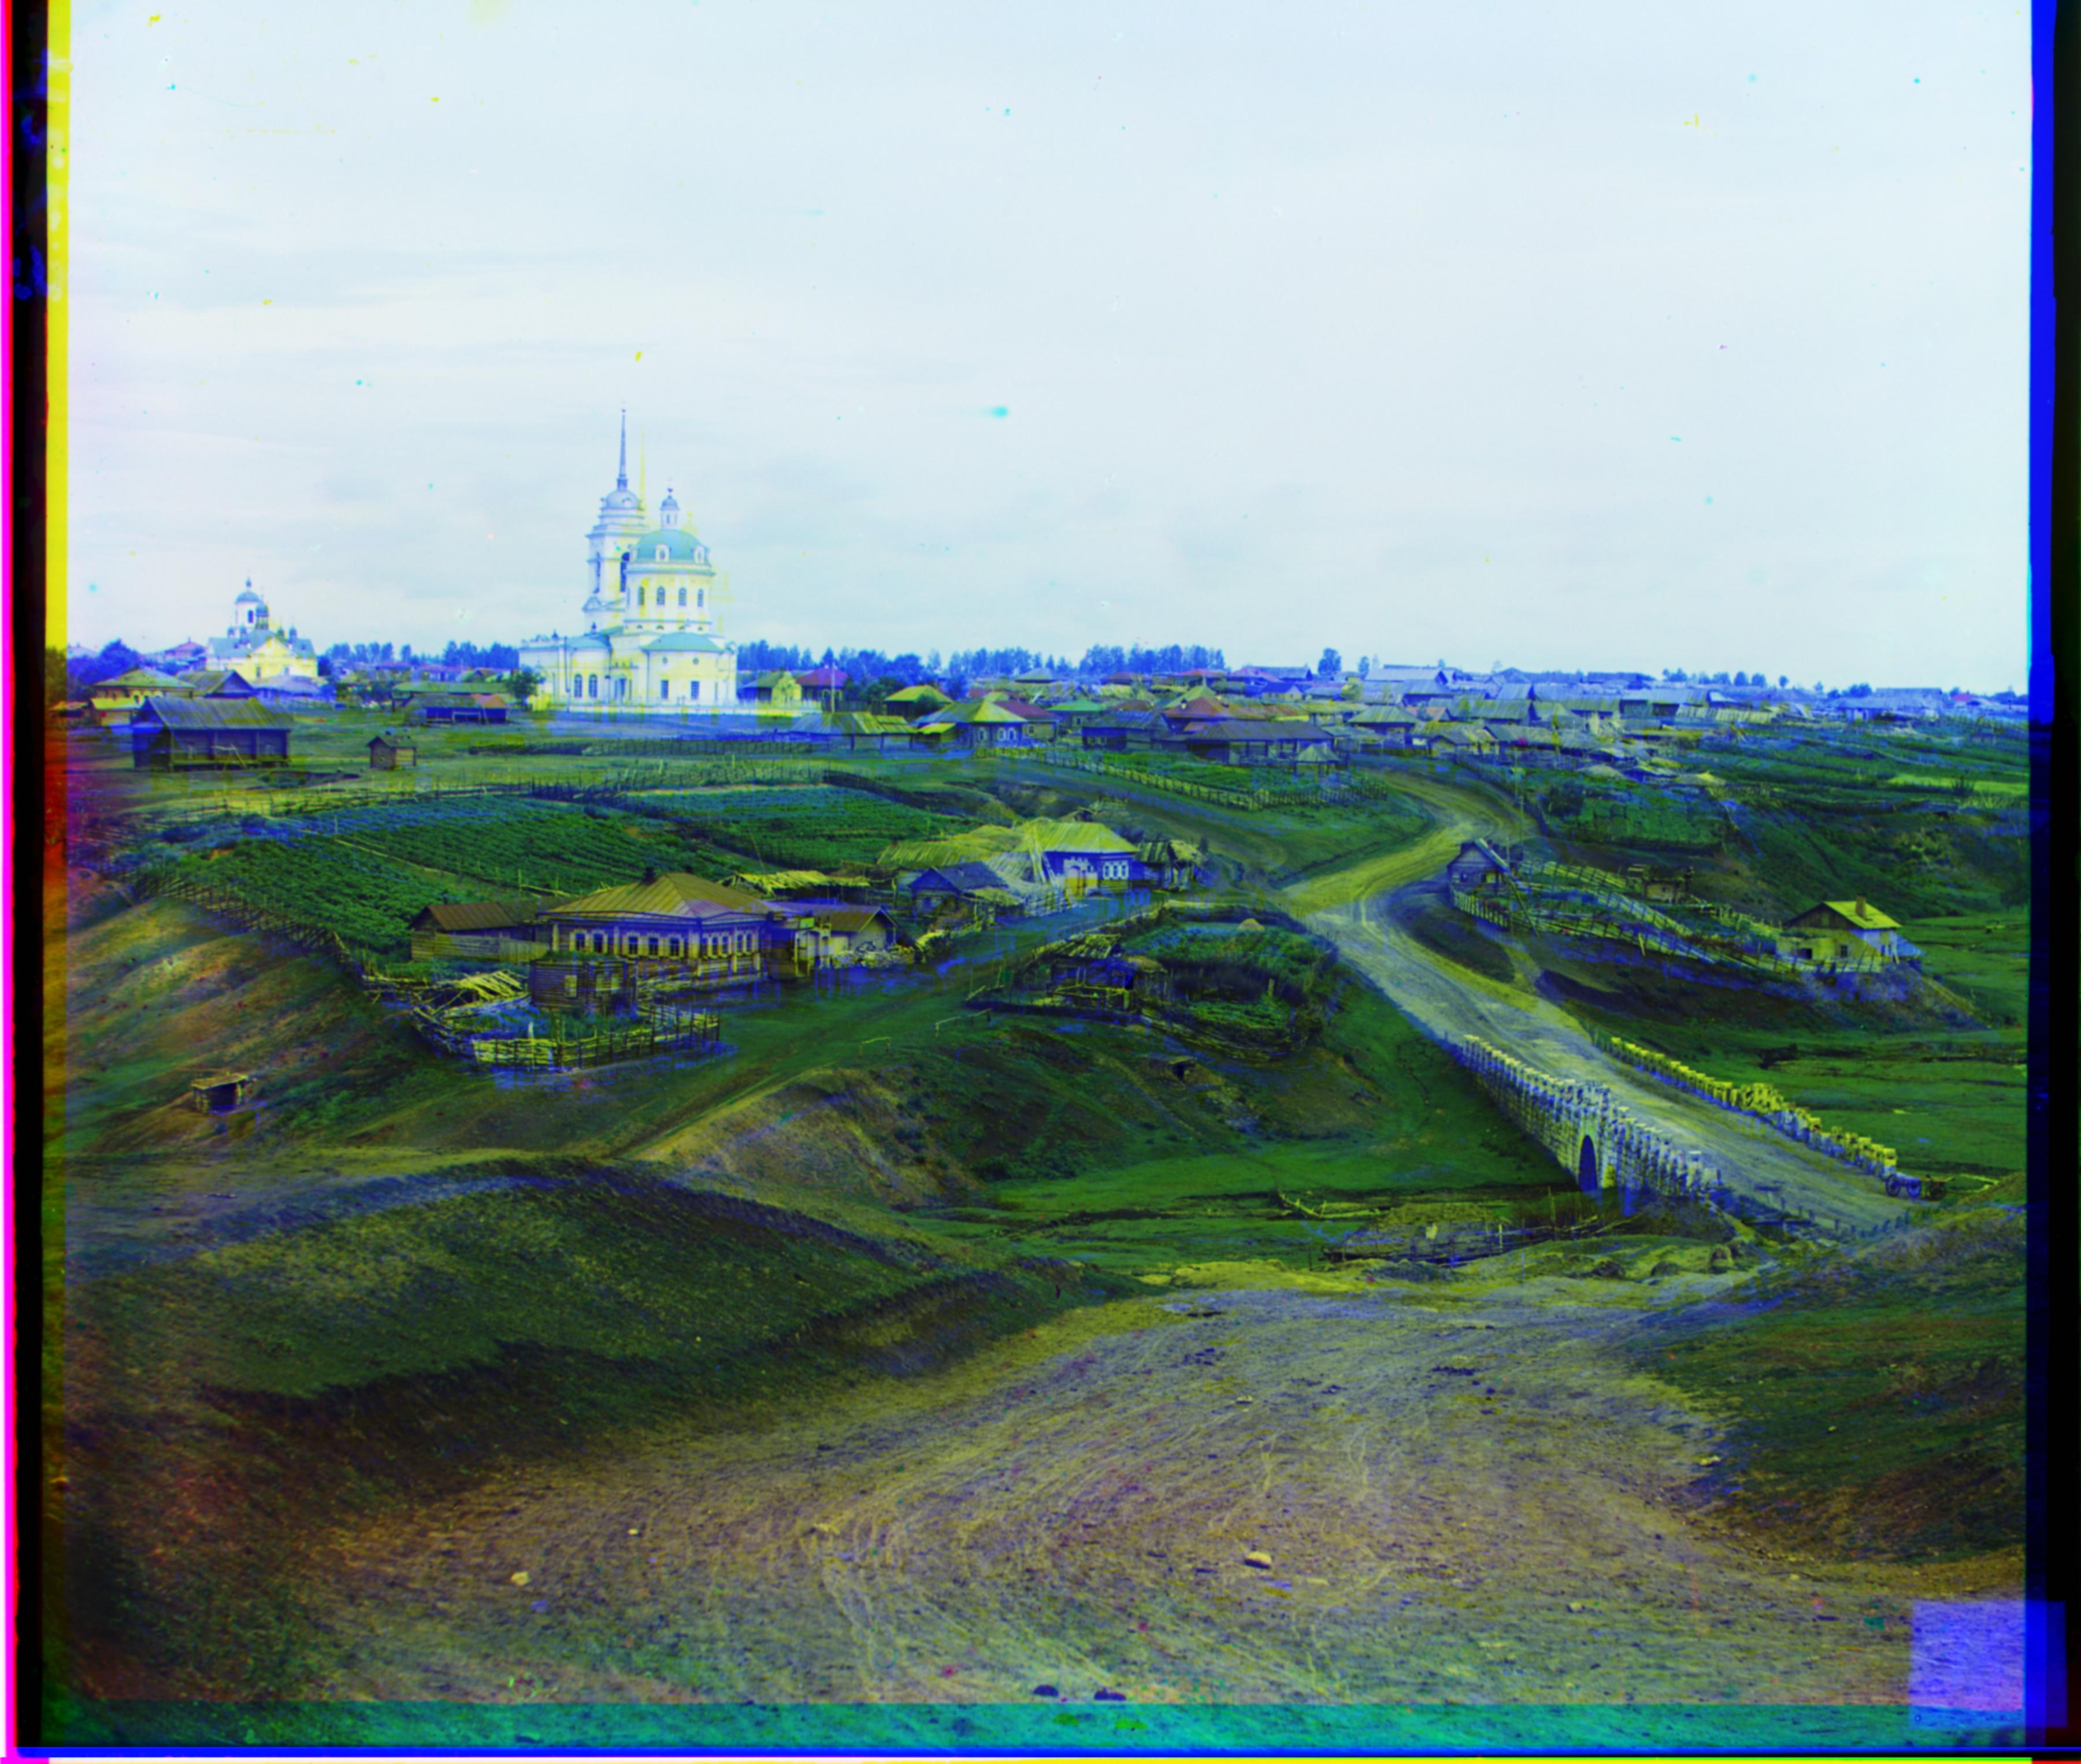
\includegraphics[width=\textwidth,height=\textheight,keepaspectratio]{../output/large-images/villag-aligned.jpg}
\caption{Aligned image for village.tif  size = 3601 x 3053}
\end{figure}



























\end{document}